\documentclass[11pt]{article}
\usepackage{tikz}
\usepackage{forloop}
\usetikzlibrary{shadows, arrows}

% Define block styles
\tikzstyle{block} = [draw, fill=yellow!30, text width=6.0em, text centered, minimum height=1.5em, drop shadow]
\tikzstyle{blockNms} = [draw, fill=blue!15, text width=4.0em, text centered, minimum height=1.5em, drop shadow]
\tikzstyle{blockPre} = [draw, fill=cyan!20, text width=4.0em, text centered, minimum height=1.5em, drop shadow]
\tikzstyle{blockCat} = [draw, fill=cyan!20, text width=4.0em, text centered, minimum height=1.5em, drop shadow]
\tikzstyle{layer} = [block, text width=10em, minimum width=14em, minimum height=3em, rounded corners, drop shadow]
\tikzstyle{layerNms} = [blockNms, text width=10em, minimum width=10em, minimum height=3em, rounded corners, drop shadow]
\tikzstyle{layerPre} = [blockPre, text width=10em, minimum width=10em, minimum height=3em, rounded corners, drop shadow]
\tikzstyle{layerCat} = [blockCat, text width=10em, minimum width=10em, minimum height=3em, rounded corners, drop shadow]
\tikzstyle{line} = [draw, thick, color=black!90, -latex']
\tikzstyle{ur}=[draw, color=red!40, text centered, minimum height=0.01em]

% Draw layer
\newcommand{\layer}[2]{
node (l#1) [layer] {#2}}

\newcommand{\layerNms}[2]{
node (l#1) [layerNms] {#2}}

\newcommand{\layerPre}[2]{
node (l#1) [layerPre] {#2}}

\newcommand{\layerCat}[2]{
node (l#1) [layerCat] {#2}}

\newcommand{\arrow}[4]{
  \path [line] (#1.south) -- node [right]
    {#3, #4} (#2);}

\begin{document}
	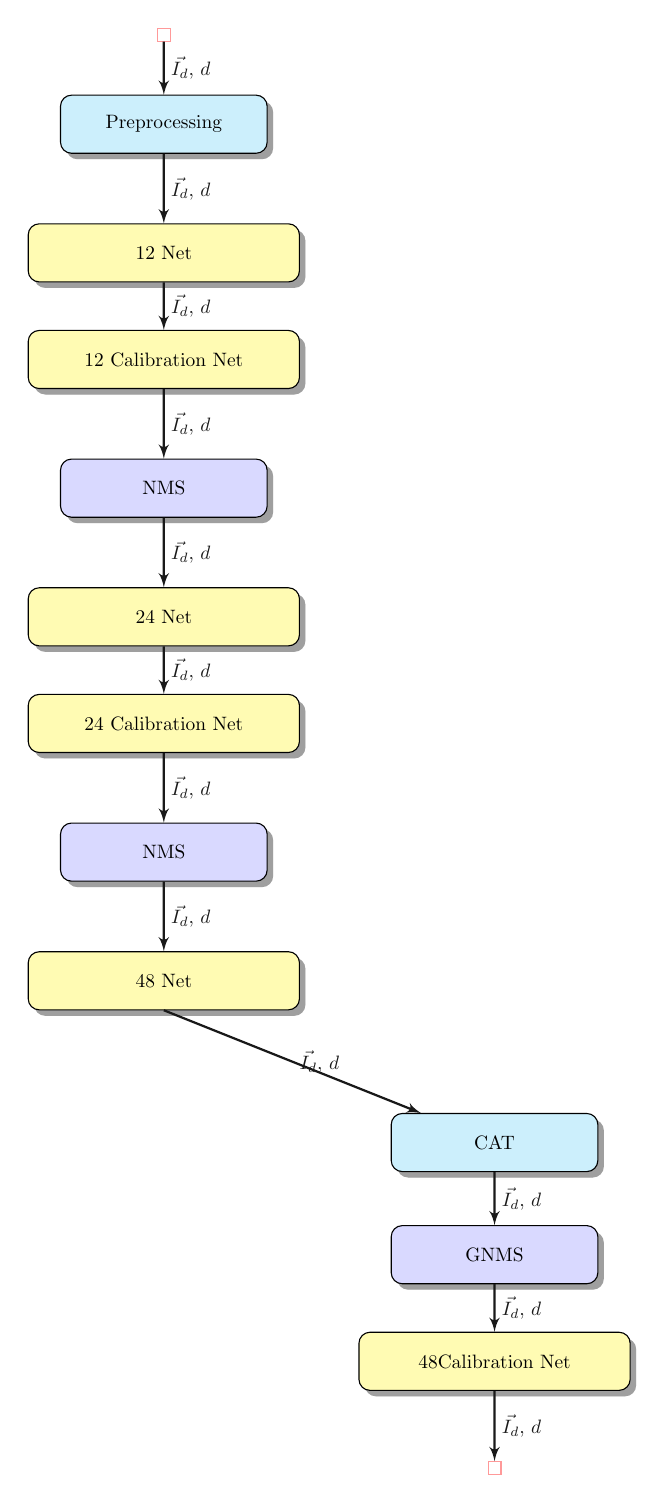
\begin{tikzpicture}[scale=0.7, transform shape]
		
		% Draw diagram elements
  		\path node (input)[ur] {};
		\path (input.south)+(0.0, -1.5) \layerPre{1}{Preprocessing};
		\path (l1.south)+(0.0, -1.8) \layer{2}{12 Net};
		\path (l2.south)+(0.0, -1.4) \layer{3}{12 Calibration Net};
		\path (l3.south)+(0.0, -1.8) \layerNms{4}{NMS};
		\path (l4.south)+(0.0, -1.8) \layer{5}{24 Net};
		\path (l5.south)+(0.0, -1.4) \layer{6}{24 Calibration Net};
		\path (l6.south)+(0.0, -1.8) \layerNms{7}{NMS};
		\path (l7.south)+(0.0, -1.8) \layer{8}{48 Net};
		\path (l8.south)+(6.0, -2.4) \layerCat{9}{CAT};
		\path (l9.south)+(0.0, -1.5) \layerNms{10}{GNMS};
		\path (l10.south)+(0.0, -1.4) \layer{11}{48Calibration Net};
  		\path (l11.south)+(0.0, -1.4) node (output)[ur] {};
		
		% Draw arrows between elements
		\arrow{input}{l1}{$\vec{I_d}$}{$d$};
		\arrow{l1}{l2}{$\vec{I_d}$}{$d$};
		\arrow{l2}{l3}{$\vec{I_d}$}{$d$};
		\arrow{l3}{l4}{$\vec{I_d}$}{$d$};
		\arrow{l4}{l5}{$\vec{I_d}$}{$d$};
		\arrow{l5}{l6}{$\vec{I_d}$}{$d$};
		\arrow{l6}{l7}{$\vec{I_d}$}{$d$};
		\arrow{l7}{l8}{$\vec{I_d}$}{$d$};
		\arrow{l8}{l9}{$\vec{I_d}$}{$d$};
		\arrow{l9}{l10}{$\vec{I_d}$}{$d$};
		\arrow{l10}{l11}{$\vec{I_d}$}{$d$};
		\arrow{l11}{output}{$\vec{I_d}$}{$d$};
		
	\end{tikzpicture}
\end{document}
